\documentclass{article}
\usepackage[utf8]{inputenc}
\usepackage{amsmath}
\usepackage{hyperref}
\usepackage{graphicx}
\usepackage{fancyhdr}
\usepackage[a4paper, total={6in, 8in}]{geometry}
\usepackage{enumitem}
\usepackage{amsfonts}

\pagestyle{fancy}
\fancyhf{}
\lhead{Ian Chow}
\rhead{CTA200 Assignment 3 Part 3}

\begin{document}

\section*{Question 1}

\subsection*{Methods}
In this question, we found the set of complex values $c$, for which the initial condition $z_0 = 0$ does not cause the quadratic map $z_{i + 1} = z_i + c$ to diverge to infinity. To do this, we generated a square grid of points $c = xi + y$ in the complex plane, with the boundaries $|x|, |y| \leq 2$. We then wrote a Python function called \texttt{quad\_map\_colouring()} to determine whether any given value of $c$ causes the quadratic map to eventually leave the boundaries noted above. It performs this task by iterating over the quadratic map over a maximum number of iterations ($100$ in our analysis) for each point $c$ in the grid, and checking whether $|\mathfrak{R}(z_i)| > 2$ or $|\mathfrak{I}(z_i)| > 2$ at the $i$th iteration to determine whether the map has diverged, returning the current value of $i$ if so. Otherwise, if it completes the maximum number of iterations without detecting divergence, it concludes that the point stays bounded and returns the value $-1$. 
\smallbreak
We then implemented a list comprehension in Python, iterating \texttt{quad\_map\_colouring()} over all the points in the grid to assign them each a numerical value depending on whether they diverge or not as detailed above. 

\subsection*{Results}
To plot the first graph (points that diverge are coloured white while points that stay bounded are coloured black), we simply coloured any points assigned the value $-1$ (bounded) as black and all other points as white. The results of this plot are shown in Fig. \ref{fig:quad_map_bw}:

\begin{figure}
    \hspace{-15mm}
    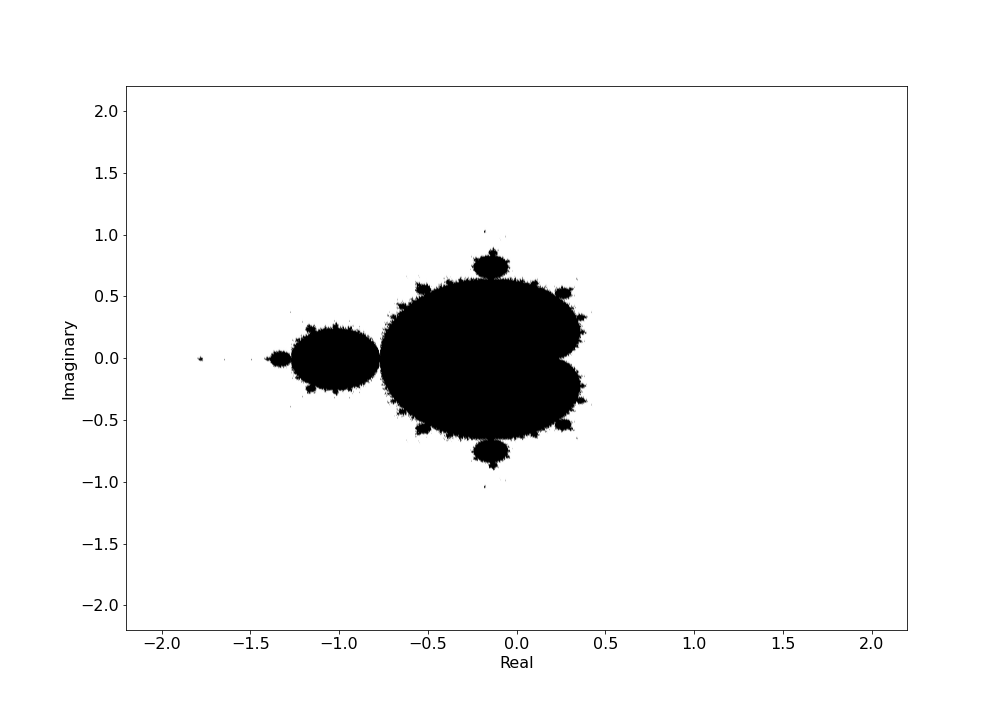
\includegraphics[scale=0.6]{quad_map_colouring_bw.png}
    \caption{A plot showing the set of divergent points $c$ in the complex plane, for the quadratic map $z_{i + 1} = _i + c$ with initial condition $z_0$. Points for which the map diverges beyond $|\mathfrak{R}(z_i)| > 2$ or $|\mathfrak{I}(z_i)| > 2$ are coloured in white, while points for which the map stays bounded within $|\mathfrak{R}(z_i)| \leq 2$ or $|\mathfrak{I}(z_i)| \leq 2$ are coloured in black.}
    \label{fig:quad_map_bw}
\end{figure}

To plot the second graph (points coloured by a colourscale indicating the iteration number at which the point diverged) we used Matplotlib's built-in \texttt{plt.colorbar()} function to display a colorbar ranging from dark blue to white on the right of the graph. To increase contrast, all points which took $\geq 25$ iterations (near the boundary of the set) are assigned the same colour (white). The points which did not diverge (assigned $-1$) were given a very dark blue colour. The results of the second plot are shown in Fig. \ref{fig:quad_map_scale}:
\begin{figure}
    \hspace{-15mm}
    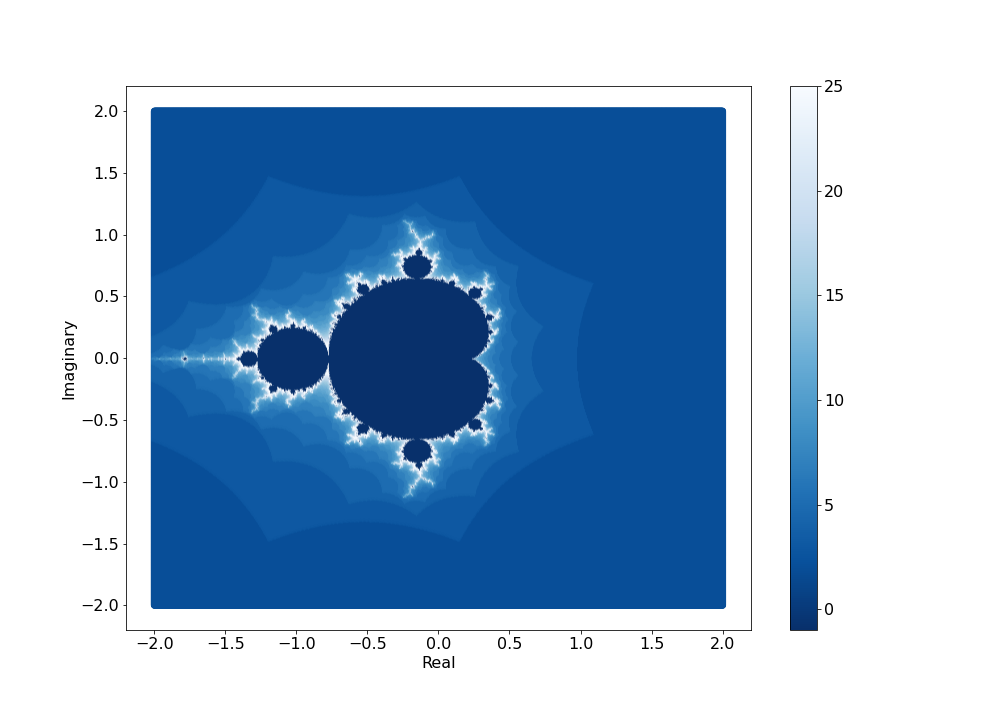
\includegraphics[scale=0.6]{quad_map_colouring_scale.png}
    \caption{A plot showing the set of divergent points $c$ in the complex plane for the quadratic map for the quadratic map $z_{i + 1} = _i + c$ with initial condition $z_0$. Points are coloured according to the iteration number $i$ at which $z_i$ diverges for that value of $c$. Values of $z_i$ that remain bounded are coloured with a very dark blue and form the central cardioid of the plot.}
    \label{fig:quad_map_scale}
\end{figure}
\smallbreak
Note that the results of both plots are the Mandelbrot set, as expected. We can see that the system exhibits chaotic behaviour near the edges of the set (small changes in $c$ can result in changes to the stability of the map).

\newpage
\section*{Question 2}

\subsection*{Methods}

In this question, we found numerical solutions to Lorenz's equations using the parameters given in the original paper, reproducing his results. We first wrote a function \texttt{lorenz\_equations()} to implement Lorenz's equations, given by:

\begin{eqnarray}
\dot X &=& -\sigma(X-Y)\\ \nonumber
\dot Y &=& rX -Y - XZ\\ \nonumber
\dot Z &=& -bZ + XY \nonumber
\end{eqnarray}
where $\sigma$, $r$, and $b$ are empirically determined dimensionless parameters.We then used SciPy's \texttt{scipy.integrate.solve\_ivp()} function to numerically integrate Lorenz's equations from $t = 0$ to $t = 60$ (in dimensionless time units), using the starting condition $W_0 = [X_0, Y_0, Z_0] = [0, 1, 0]$ and parameters $\sigma = 10$, $r = 28$ and $b = 8/3$. Using a time scale of $\Delta t = 0.01$ for each iteration (as in Lorenz's paper), we then plotted the time evolution of $Y$ over the first $3000$ iterations of Lorenz's equations to reproduce his Figure 1 in the original paper.
\smallbreak
We then also plotted $X$ against $Y$ and $Y$ against $Z$ from iterations $1400 - 1900$ to reproduce Lorenz's Figure 2 as well. Finally, we repeated our numerical integration with the same parameters $\sigma, r, b$, but with different starting conditions of $W_0' = W_0 + [0, 10^{-8}, 0]$ instead. Since the system is chaotic, we expect $W'$ to diverge from $W$ exponentially. We thus calculated the distance between the computed values of the $W'(t)$ and $W(t)$ vectors (since $W(t) = [X(t), Y(t), Z(t)]$, using the $L^2$ norm definition of distance for both $W(t)$ and $W'(t)$), and plotted $||W'(t) - W(t)||$ against time.

\subsection*{Results}

The results of the first graph (Lorenz's Fig. $1$) can be found in our Fig. \ref{fig:lorenz_1}, in which we plotted the results of $Y$ for the first $3000$ iterations. Note that as in Lorenz's Fig. 1, the first row is the first $1000$ iterations, the second row are iterations $1000$ to $2000$, and the third row are iterations $2000$ to $3000$.

\begin{figure}
    \hspace{-25mm}
    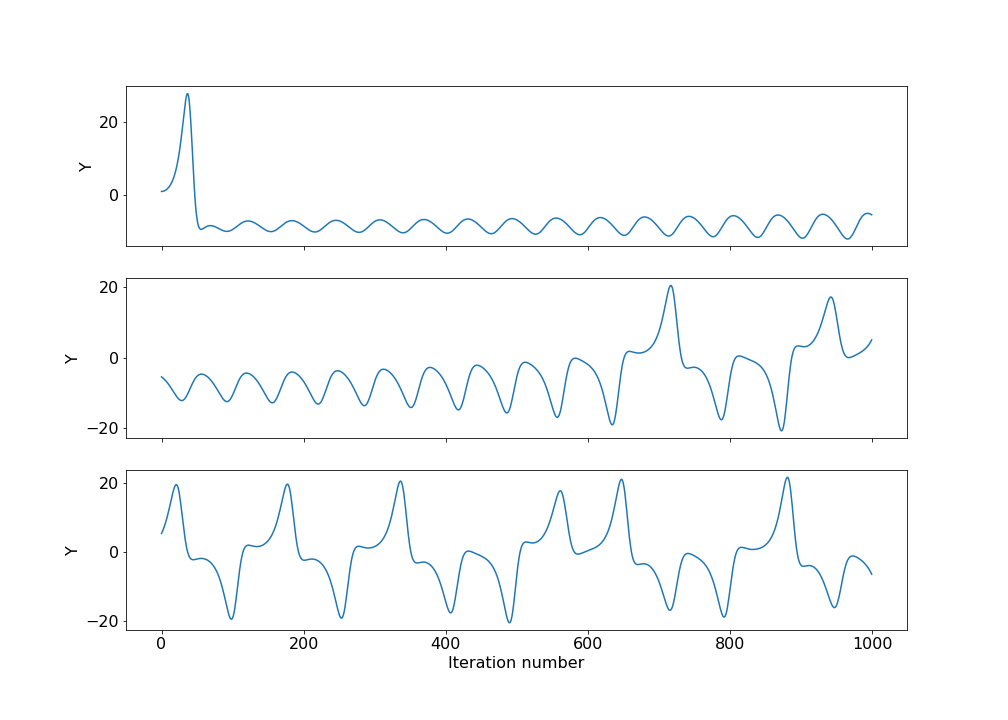
\includegraphics[scale=0.6]{lorenz_fig_1.png}
    \caption{Plot showing the evolution of $Y$ over $3000$ iterations. Similar to Lorenz's paper, we can see an initial peak early in the first $1000$ iterations, followed by oscillations that gradually incrase in amplitude until $Y$ crosses $0$ near iteration $1700$ at which it changes sign. It then changes sign numerous times for the rest of the iterations.}
    \label{fig:lorenz_1}
\end{figure}

Similarly, the results of the second graph (Lorenz's Fig. $2$ can be found in our Fig. \ref{fig:lorenz_2}, in which we plotted $Y$ against $Z$ and $X$ against $Y$ from iterations $1400 - 1900$. 

\begin{figure}
    \hspace{-15mm}
    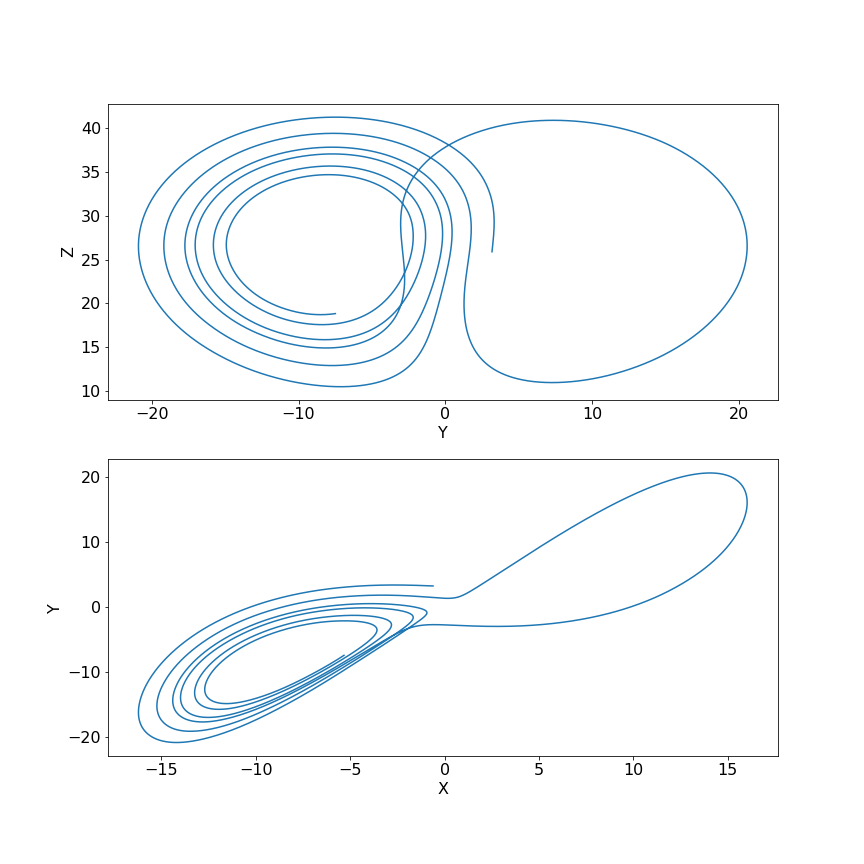
\includegraphics[scale=0.6]{lorenz_fig_2.png}
    \caption{Plot showing the evolution of $X$ vs. $Y$ and $Y$ vs. $Z$ from iterations $1400$ to $1900$. Similar to Lorenz's plot, we can see characteristic concentric orbits around stable fixed points $C$ and $C'$.}
    \label{fig:lorenz_2}
\end{figure}

Finally, a plot of the distance (dimensionless) between $W'$ and $W$ over time is shown in Fig. \ref{fig:w_prime_distance}. Note that the $y$-scale (distance) is logarithmic, and the system originally starts with a distance of $10^{-8}$ (based on the distance between $W_0$ and $W_0'$). The distance appears to increase as roughly a straight line (with some oscillations) between $t \approx 20$ and $t \approx 40$, showing exponential growth in that region, as predicted by Lorenz.

\begin{figure}
    \hspace{-25mm}
    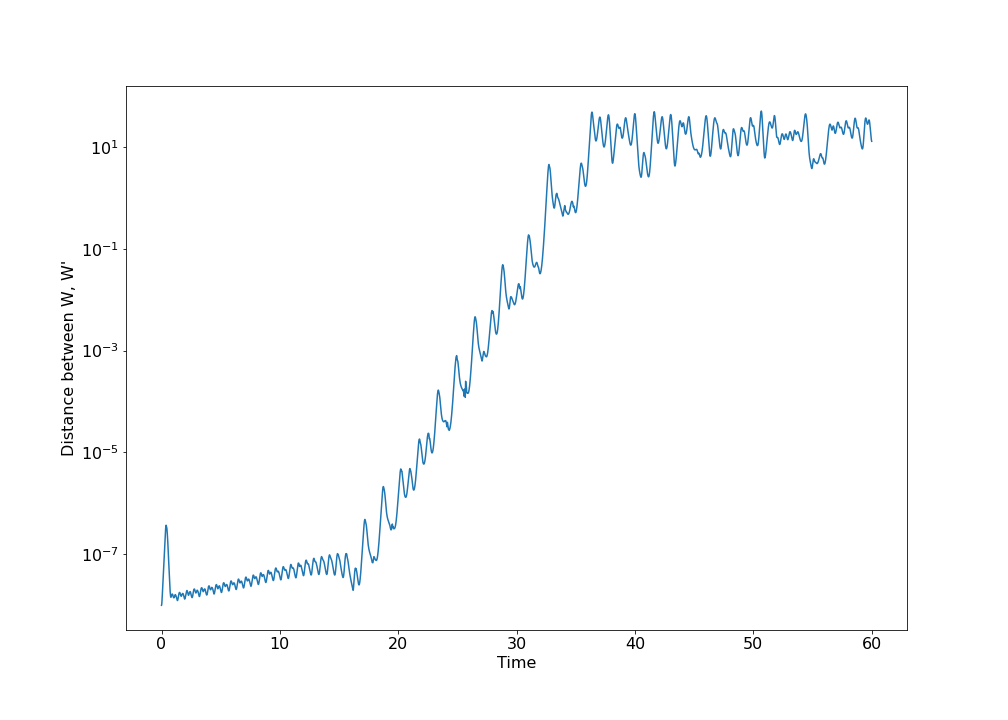
\includegraphics[scale=0.6]{w_prime_distance.png}
    \caption{Plot of the distance (as calculated by $L^2$ norm) between $W$ and $W'$ over time from $t = 0$ to $t = 60$. Note that $||W_0 - W_0'|| = 10^{-8}$. Disregarding oscillations, the distance appears to grow slowly (sub-exponential) initially during the oscillatory period at the beginning (as shown in Fig. $1$), before increasing exponentially as the systems begin to experience instability. Finally, the distance appears to reach a maximum of about $\sim 10^1$ as both systems become totally chaotic.}
    \label{fig:w_prime_distance}
\end{figure}

\end{document}